\documentclass[times, utf8, seminar, numeric]{fer}

\usepackage{booktabs}
\usepackage{hyperref}
\usepackage{enumitem}
\usepackage{mathtools}
\usepackage{listings}
\usepackage{multirow}
\usepackage{tikz}
\usepackage{svg}
\usepackage{listings}
\usepackage[croatian,boxed,noline]{algorithm2e}
\SetKwProg{Fn}{Funkcija}{}{}

\definecolor{dkgreen}{rgb}{0,0.6,0}
\definecolor{gray}{rgb}{0.5,0.5,0.5}
\definecolor{mauve}{rgb}{0.58,0,0.82}

% ovo su postavke za kod
\lstset{frame=tb,
  language=Python,
  aboveskip=3mm,
  belowskip=3mm,
  showstringspaces=false,
  columns=flexible,
  basicstyle={\small\ttfamily},
  numbers=left,
  numberstyle=\tiny\color{gray},
  keywordstyle=\color{blue},
  commentstyle=\color{dkgreen},
  stringstyle=\color{mauve},
  breaklines=true,
  breakatwhitespace=true,
  tabsize=3
}

\renewcommand{\lstlistingname}{Isječak koda}% Listing -> Isječak koda

\begin{document}

\title{Izgradnja binarnog stabla valića kao RRR strukture}
\author{Mislav Magerl, Matija Milišić, Mateo Šimonović}
\voditelj{izv. prof. dr. sc. Mile Šikić}

\maketitle

\tableofcontents

\chapter{Uvod}
alo

\chapter{RRR struktura}
\label{sec:rrr}
RRR struktura je podatkovna struktura koja se koristi za brze rank, select te access upite nad binarnim nizom znakova. RRR strukturu su predložili Raman, Raman and Rao \citep{DBLP:journals/corr/abs-0705-0552} te je po njima i dobila ime. Metoda $rank(i)$ odgovara na pitanje koliko se jedinica nalazi u ulaznom nizu do, uključivo, indeksa $i$. Metoda $select(i)$ odgovara na pitanje na kojem se indeksu u ulaznom nizu nalazi $i$-ta jedinica. Metoda $access(i)$ odgovara koji znak se nalazi na indeksu $i$ u ulaznom nizu - nula ili jedinica.

\section{Izgradnja strukture}
\label{sec:izgradnja-rrr}
Ulazni binarni niz podijeljen je u blokove, a blokovi su podijeljeni u superblokove. Broj znakova u bloku ($b$) te broj blokova u superbloku ($f$) su parametri strukture. Na slici \ref{fig:rrr} prikazan je primjer RRR strukture s parametrima $b=5$ te $f=2$. Ako nisu eksplicitno zadani, parametri se računaju u ovisnosti o veličini ulaznog niza ($n$):
$b=\frac{\log_2n}{2}$,
$f=2  \log_2n$.
Svaki blok struktura pamti par vrijednosti - klasu \engl{class} - $c$ i pomak \engl{offset} - $o$. Klasa je broj jedinica u bloku, a pomak je indeks permutacije jedinica u lookup tablici koja je zadjednička za cijelu strukturu. 

\textbf{Lookup tablica}

Lookup tablica sadrži $2^b$ redova. Svaki red prikazuje jednu od mogućih različitih blokova veličine $b$ - sve kombinacije nula i jedinica u nizu veličine $b$. Dodatno, tablica je na taj način izgrađena da su prvo sve permutacije s nula jedinica, zatim sve permutacije s jednom, dvije te naposlijetku $b$ jedinica. Za svaki zapis zapisan je niz kumulativne sume do $i$-tog elementa u tom bloku. Dio lookup tablice prikazan je na slici \ref{fig:lookup}. Vremenska složenost izgradnje lookup tablice je $O(b \cdot 2^b)$, odnosno izraženo preko veličine ulaznog niza $O(n \cdot \log_2n)$. Memorijska složenost je također $O(b \cdot 2^b)$.

\textbf{Izgradnja strukture}

Nakon izgradnje lookup tablice za svaki blok se računa klasa i pomak te se spremaju u strukturi umjesto originalnog niza. Jedan zapis o klasi veličine je 1B iz razloga što je ukupan broj klasa $log_2b$ što za vrijednosti $b$ do $16$, odnosno vrijednosti $n$ do $10^{10}$, iznosi $4$ bita. Jedan zapis o pomaku je veličine 2B iz razloga što za svaku klasu $c$ ima $\binom{b}{c}$ zapisa, tj. maksimalno $\binom{b}{\frac{b}{2}}$. Ako se uzme da je $n$ maksimalno $10^{10}$, $b$ iznosi maksimalno $16$. Najveći pomak u nekoj klasi tada iznosi $\binom{16}{8}=12870$ za što nije potrebno više od 2B.  Ukupno se, dakle, za jedan blok troši 3B memorije. Ukupna memorijska složenost je $O(\frac{n}{b})$, odnosno izraženo samo preko veličine niza $O(\frac{n}{log_2n})$
Također, struktura pamti i kumulativnu sumu do svakog superbloka. Memorijska složenost te sume je $O(frac{n}{b f})$, odnosno izraženo samo preko veličine niza $O(\frac{n}{(\log_2n)^2})$.

\begin{figure}[ht]
	\centering
	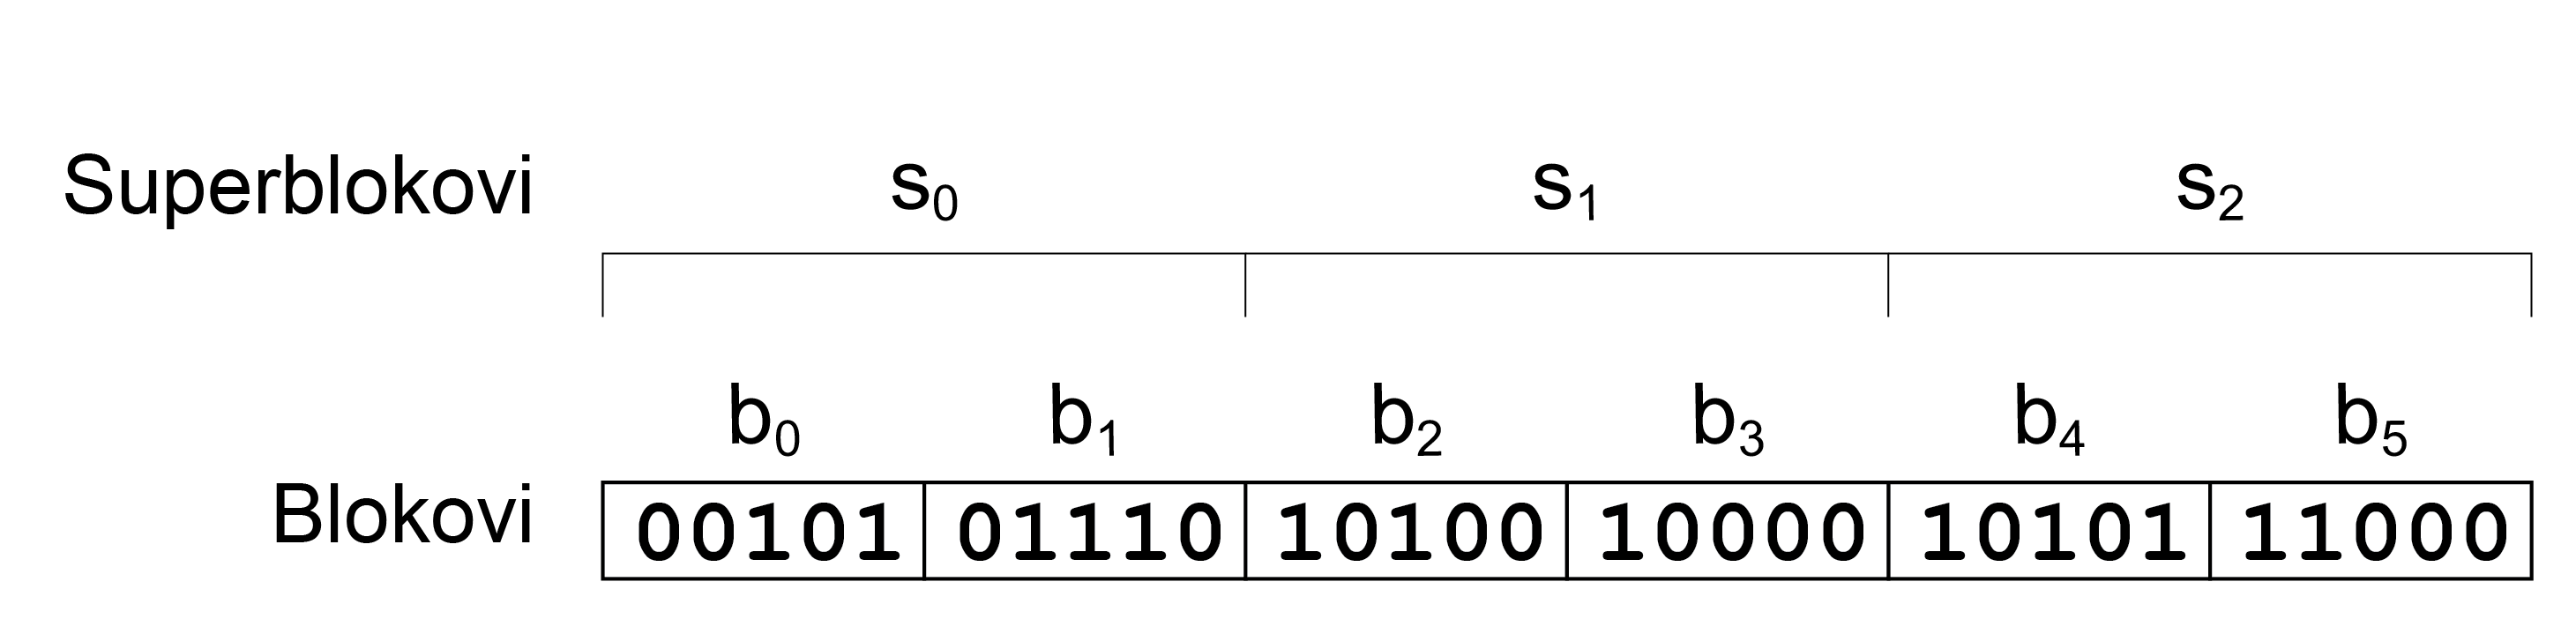
\includegraphics[width=15cm]{img/rrr_blocks.png}
	\caption{Prikaz blokova i superblokova RRR strukture}
	\label{fig:rrr}
\end{figure}

\begin{figure}[ht]
	\centering
	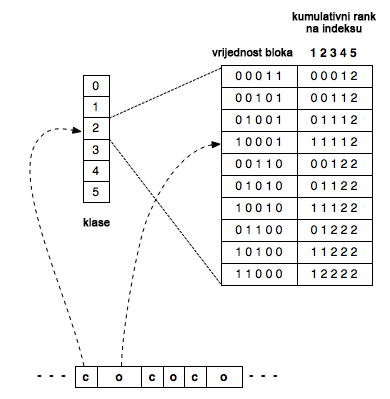
\includegraphics[width=10cm]{img/rrr-binary-table.png}
	\caption{Prikaz lookup tablice unutar RRR strukture}
	\label{fig:lookup}
\end{figure}


\section{Operacije nad sturkturom}
U sljedećim odlomcima bit će opisane implementacije operacija $rank$, $select$ i $access$ nad RRR strukturom.


\subsection{Rank}
U RRR strukturi postoje dvije rank operacije - $rank_0(i)$ te $rank_1(i)$. Operacija $rank_0(i)$ vraća broj nula do, uključivo, indeksa $i$, a $rank_1(i)$ broj jedinica do indeksa. 
Jedna metoda može se vrlo jednostavno izraziti pomoću druge. Tako implementacija metode $rank_0(i)$ izgleda ovako:


\begin{algorithm}[H]
 \caption{Pseudokod metode $rank_0$}
 \Fn{\texttt{rank0(i)}}{
	\Vrati \texttt{i + 1 - rank1(i)}\;

 }
\end{algorithm}


Operacija $rank_1(i)$ se računa na sljedeći način:
\begin{enumerate}
	\item Izračuna se indeks superbloka te bloka u kojem se pozicija $i$ nalazi
	\item Izračuna se suma svih blokova do bloka u kojem se pozicija $i$ nalazi
	\item Pomoću lookup tablice se na sumu dodaje suma brojeva do pozicije $i$
\end{enumerate}
Pseudokod:

\begin{algorithm}[H]
 \caption{Pseudokod metode $rank_1$}
 \Fn{\texttt{rank1(i)}}{
 	\texttt{indexBloka = i / b\;
	indexSuperbloka = i / (b*f)\;
	rez = kumulativnaSumaSuperbloka(indexSuperbloka - 1)\;
	\Za {\texttt{i = indexSuperbloka * f .. indeksBloka}}{
		rez += klasa[i]\;
	}
	c = klasa[indexBloka]\;
	o = pomak[indexBloka]\;
	rez += lookup[c][o][index - indexBloka * b]\;
	\Vrati rez;}

 }
\end{algorithm}

Složenost rank operacija je $O(f)$, odnosno $O(log_2n)$.

\subsection{Select}
Kao i za rank operaciju i select operacija ima svoje dvije varijante - $select_0(i)$ te $select_1(i)$ koje vraćaju indeks $i$-tog pojavljivanja nule odnosno jedinice. Te dvije metode mogu se napisati općenito, jednom funkcijom koja kao parametar prima boolean parametar koji određure traži zove li se $select_0$ ili $select_1$.
Operacija $select_1(i)$ računa se na sljedeći način:
\begin{enumerate}
	\item Pronađi binarnim pretraživanjem superblok u kojem se nalazi tražena jedinica
	\item U brojač pohrani sumu jedinica do prethodnog superbloka
	\item Dodaj u brojač blokove sve dok ne dođeš do bloka koji prethodi bloku u kojem je tražena jedinica
	\item Binarnim pretraživanjem pronađi poziciju tražene jedinice u bloku.
\end{enumerate}
Pseudokod:

\begin{algorithm}[H]
 \caption{Pseudokod metode $select$}
 \Fn{\texttt{select(i, tip)}}{
 	\texttt{indexSuperbloka = pronađiSuperblok(i, tip)\;
	brojač = kumulativnaSumaSuperbloka(indexSuperbloka - 1, tip)\;
	indeksBloka = indexSuperbloka * f\;
	\Dok{\texttt{brojač < i}}{
		brojač = brojač + dohvatiKlasuBloka(indeksBloka, tip)\;
		indeksBloka = indeksBloka + 1\;
	}
	indeksBloka = indeksBloka - 1\;
	brojač = brojač - dohvatiKlasuBloka(indeksBloka, tip)\;
	indeksUBloku = pronađiIndeksUBloku(i - brojač, tip)\;
 	\Vrati indeksBloka * b + indeksUBloku\;
 	}

 }
\end{algorithm}

Metode \texttt{pronađiSuperblok}, \texttt{kumulativnaSumaSuperbloka}, \texttt{dohvatiKlasuBloka} i \texttt{pronađiIndeksUBloku} primaju kao parametar \texttt{tip}. Varijabla \texttt{tip} je istinita ako se traži jedinica, odnosno lažna ako se traži nula. Ovisno o tom parametru se metode i ponašaju. Metode \texttt{pronađiSuperblok} i \texttt{pronađiIndeksUBloku} rade binarno pretraživanje kako bi pronašle indekse.
Složenost možemo rastaviti na nekoliko dijelova. Vremenska složenost traženja superbloka je $O(\frac{n}{b \dot f})$, tj. $O(\frac{n}{(\log_2n)^2})$. Zatim se traži indeks bloka unutar superbloka - $O(f)$, tj. $O(\log_2n)$. Složenost dohvaćanja klase je konstantna, $O(1)$. Složenost traženja indeksa u bloku je $O(\log_2b)$, odnosno $O(\log_2(\log_2n))$.

\subsection{Access}
Metoda $access(i)$ vraća koji se znak nalazi na danoj poziciji - nula ili jedan. Metoda je vrlo jednostavna. Jednostavno se računa razlika između $rank1$ od trenutne pozicije i prethodne pozicije.

\begin{algorithm}[H]
 \caption{Pseudokod metode $access$}
 \Fn{\texttt{access(i)}}{
 	\texttt{\uAko{i==0}{
		\Vrati rank1(i)\;
 	} \Inace{
		\Vrati rank1(i) - rank1(i - 1)\;
 	}
 	}

 }
\end{algorithm}


\chapter{Stablo valića}
\begin{figure}[ht]
	\centering
	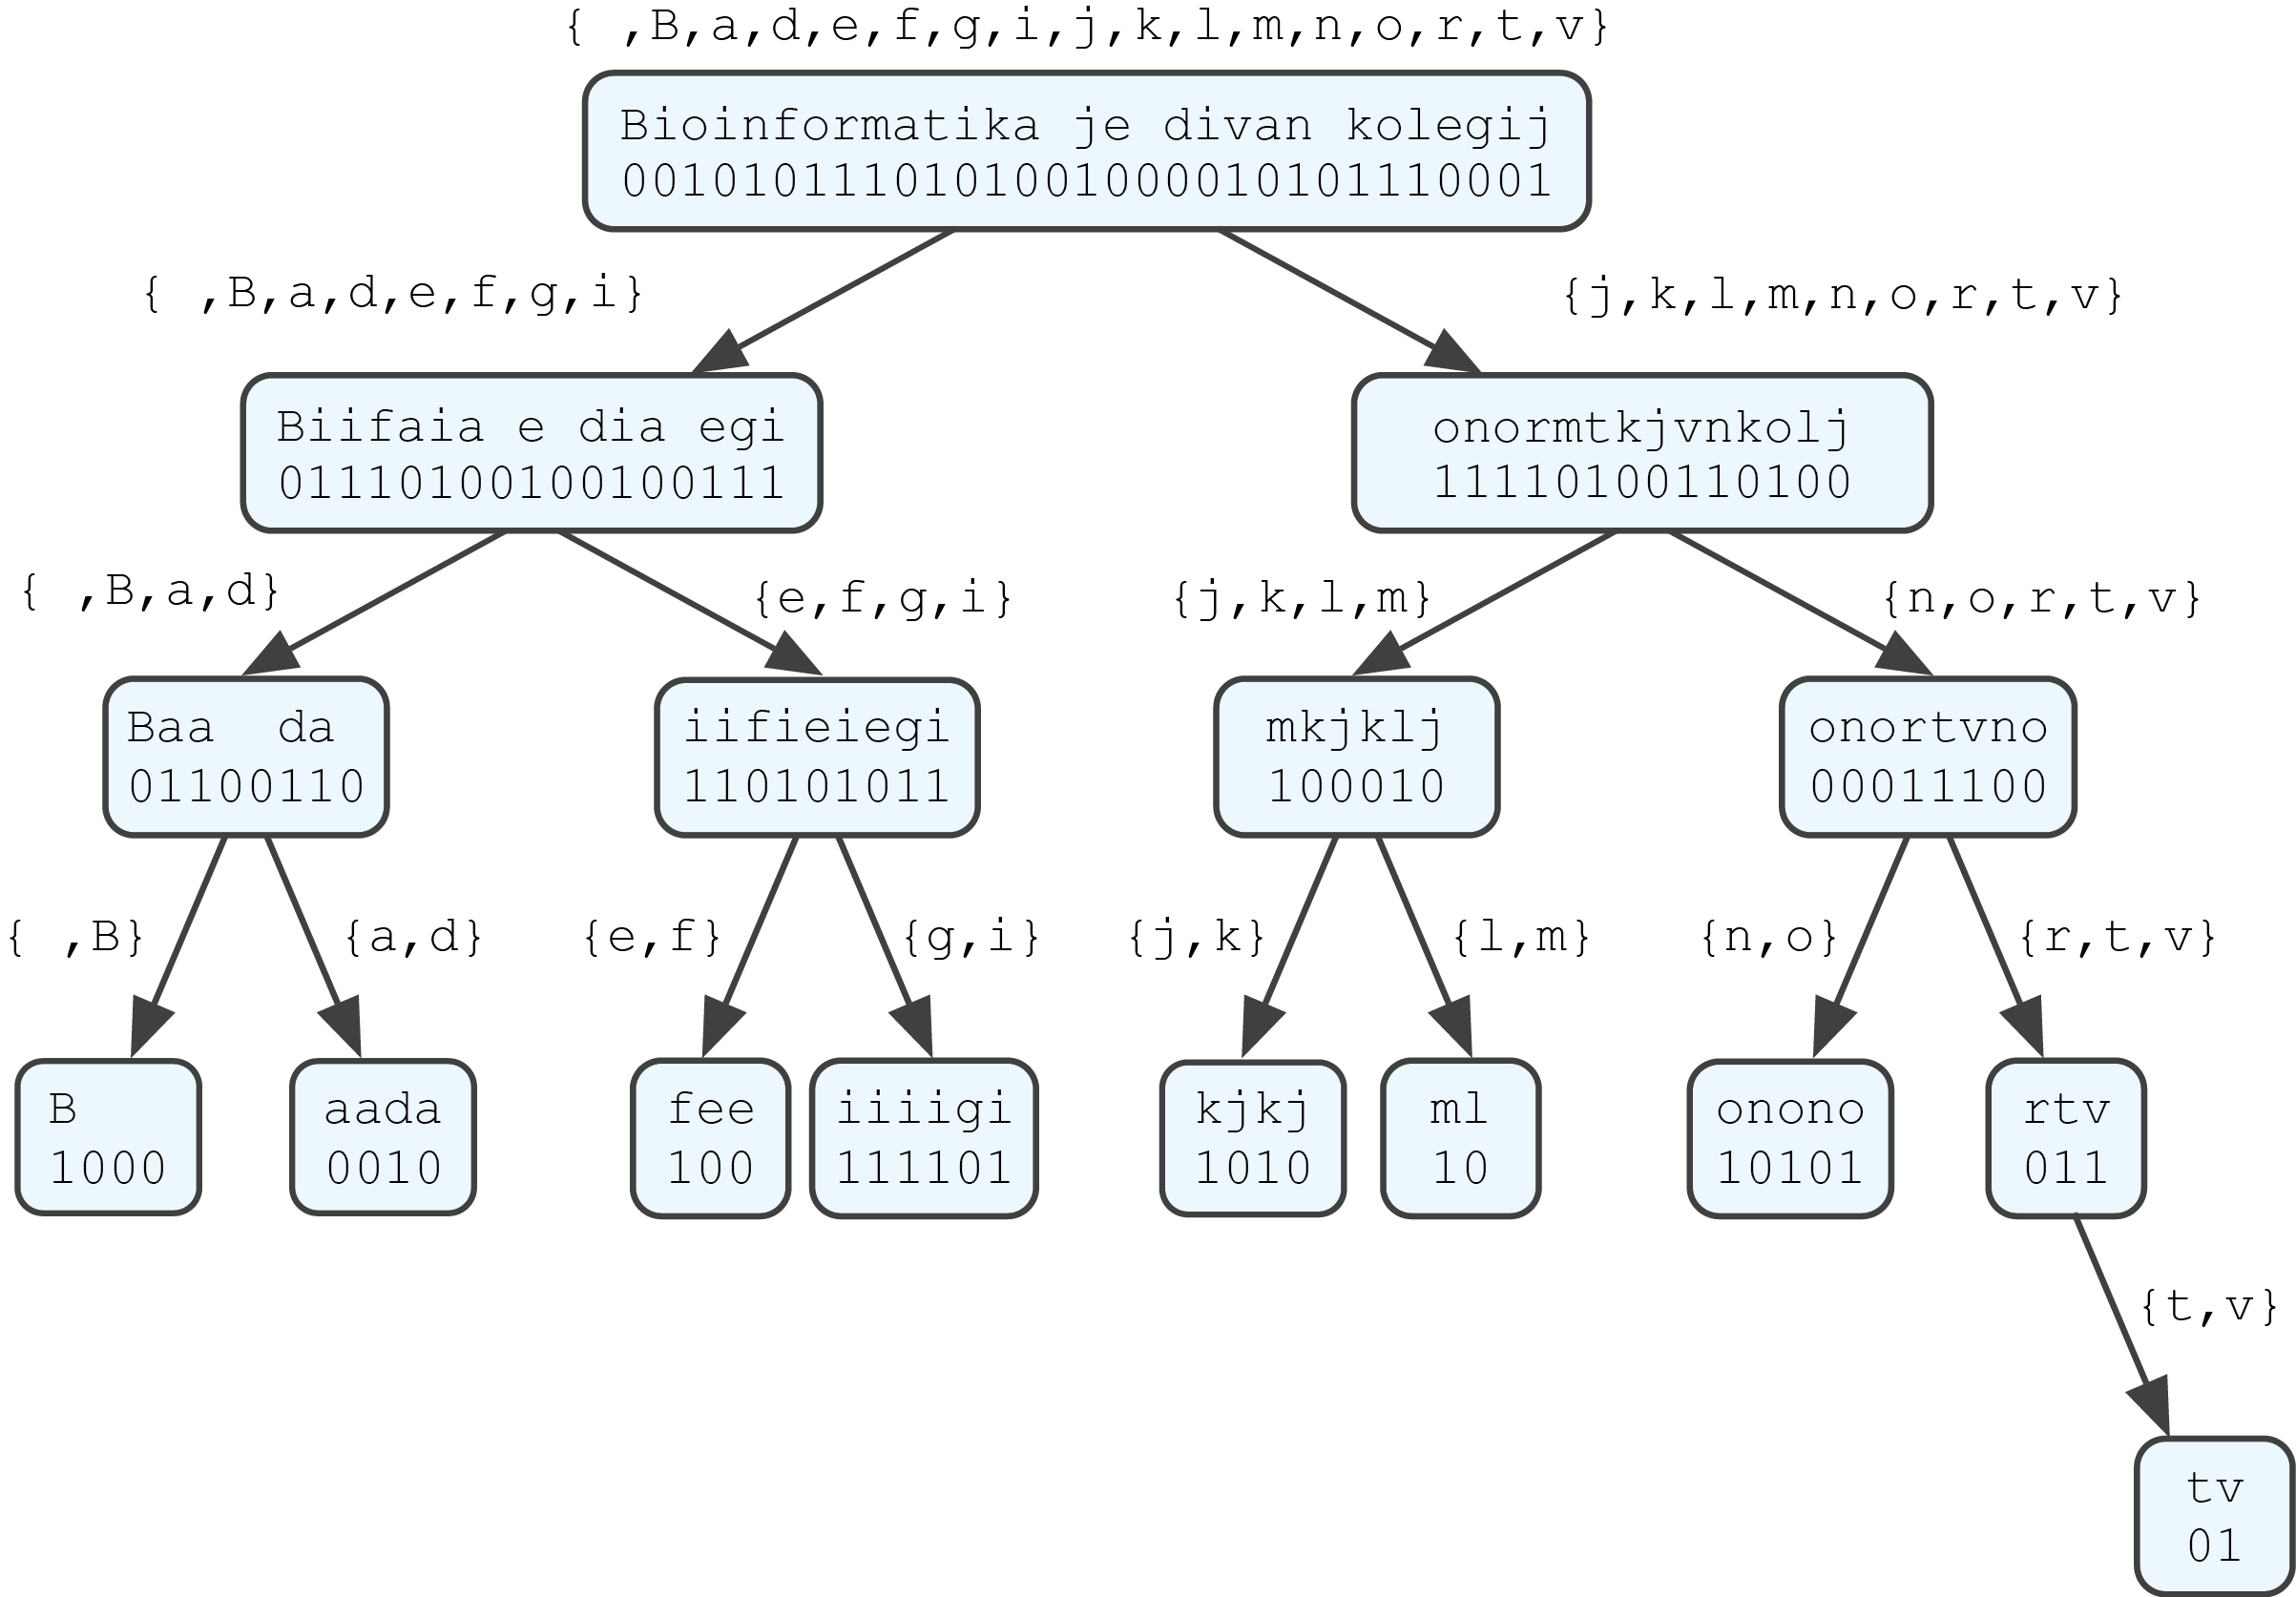
\includegraphics[width=\textwidth]{img/wavelet_tree_example.png}
	\caption{Stablo valića za ulazni niz "Bioinformatika je divan kolegij"}
	\label{fig:wavelet-tree-example}
\end{figure}



\bibliography{literature}
\bibliographystyle{fer}

\begin{sazetak}
Sazetak rada

\kljucnerijeci{Velvet}
\end{sazetak}

\end{document}
